\section{Introduction}
\IEEEPARstart{P}{roduction-line} integration for an industrial agent couples online data acquisition with governed control. The agent gathers process observations and production context, weighs them against an objective, and proposes a typed setpoint or recipe adjustment. Before any write, the runtime resolves which line, process variable, and control signal the request concerns, then applies authority and limits. In practice, a cast-film line-speed setpoint may affect measured film thickness, yet the control node and the acquisition node remain distinct even when both use Message Queuing Telemetry Transport (MQTT). Acquired observations, command acceptance, device readback, and later process measurements are therefore separate evidence, as Fig.~\ref{fig:control-path} illustrates.

One strand of research equips industrial agents for service supervision and skill-based manufacturing \cite{biskupovic2025supervision,koehle2026llmdriven}. A second examines semantic grounding, approval, and verification for plant-facing operations, including programmable logic controller (PLC) interfaces \cite{graul2026aas,schall2026safe}, and a third treats fault-recovery planning \cite{vyas2026detection}. Building on them, we examine how an agent's online acquisition and analysis should connect to a controlled operation across task-mediated and direct entry paths. This paper examines that boundary; it claims no new control law or agent-reasoning algorithm.

Five invariants govern the design. Observations may inform an agent's proposal, but they never grant write authority, and acquisition and control mappings are direction-specific. An approved control intent is revalidated before dispatch. Command receipts, readbacks, and later process observations remain separate records, and task-mediated and direct calls converge on one guarded boundary. A scene binds line, product, recipe, and run to mappings, drivers, objectives, and limits.

The contributions are:
\begin{enumerate}
  \item A production-scene model that links context, direction-specific acquisition and control mappings, registered drivers, objectives, and limits into one agent-facing operation contract. (Section~III.)
  \item An agent-to-operation boundary in which registered harnesses acquire observations and submit control intents, while task-mediated and direct calls share one dispatcher and the applicable route-specific approval, revalidation, and write guards. (Sections~III--V.)
  \item An evidence-bounded evaluation of these mappings and governance responses, together with an exploratory simulator comparison and language-model-driven episodes. (Section~VI.)
\end{enumerate}

\begin{figure}[!b]
\centering
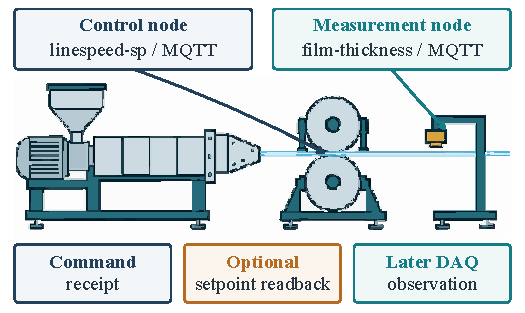
\includegraphics[width=0.98\columnwidth]{resources/fig1-vectorized-20261109.pdf}
\caption{Illustrative configured cast-film example: an agent acquires film-thickness data and may propose a line-speed adjustment, but the line-speed control node and film-thickness acquisition node remain distinct even though both use MQTT. Command acceptance or optional setpoint readback is distinct from the later process observation.}
\label{fig:control-path}
\end{figure}


